



%Autor: Nico Schrodt, Andreas Schmider
%September 2021 - Mai 2022


\documentclass[12pt]{article}

\usepackage{multicol}
\usepackage{geometry}
\usepackage{blindtext}
\usepackage{setspace}
\usepackage{hyperref}
\usepackage[headsepline=0.8pt, footsepline =0.8pt]{scrlayer-scrpage}
\usepackage{listings}
\usepackage{subcaption}
\usepackage{tabularx}
\usepackage{xurl} %Formats \url{}-entrys better
\usepackage{color, colortbl}
%\usepackage{pdfpages}
\usepackage{amssymb}
\usepackage{float}

\geometry{a4paper, top=25mm, left=35mm, right=25mm, bottom=25mm, headsep=13mm, footskip=12mm, head=14.5pt}

\lstset{mathescape=true,
        literate=
               {->}{$\rightarrow{}$}{1},
        }

%encoding
%--------------------------------------
\usepackage[utf8]{inputenc}
\usepackage[T1]{fontenc}
%--------------------------------------

%German-specific commands
%--------------------------------------
\usepackage[ngerman]{babel}
%--------------------------------------

%Hyphenation rules
%--------------------------------------
\usepackage{hyphenat}
%--------------------------------------

\usepackage{graphicx}
\usepackage{subcaption}
\graphicspath{ bilder/}

\newcommand{\Autor}{Andreas Schmider, Nico Schrodt}

\newcommand{\Bearbeitungszeitraum}{2 Semester}
\newcommand{\Kurs}{TINF19B3}
\newcommand{\Betreuer}{Prof. Dr.-Ing. Kai Becher}

\newcommand{\DHBWLogoDeckblatt}{
\includegraphics[width=4.5cm]{Logos/dhbw-logo}}
\newcommand{\IntelDataLines}{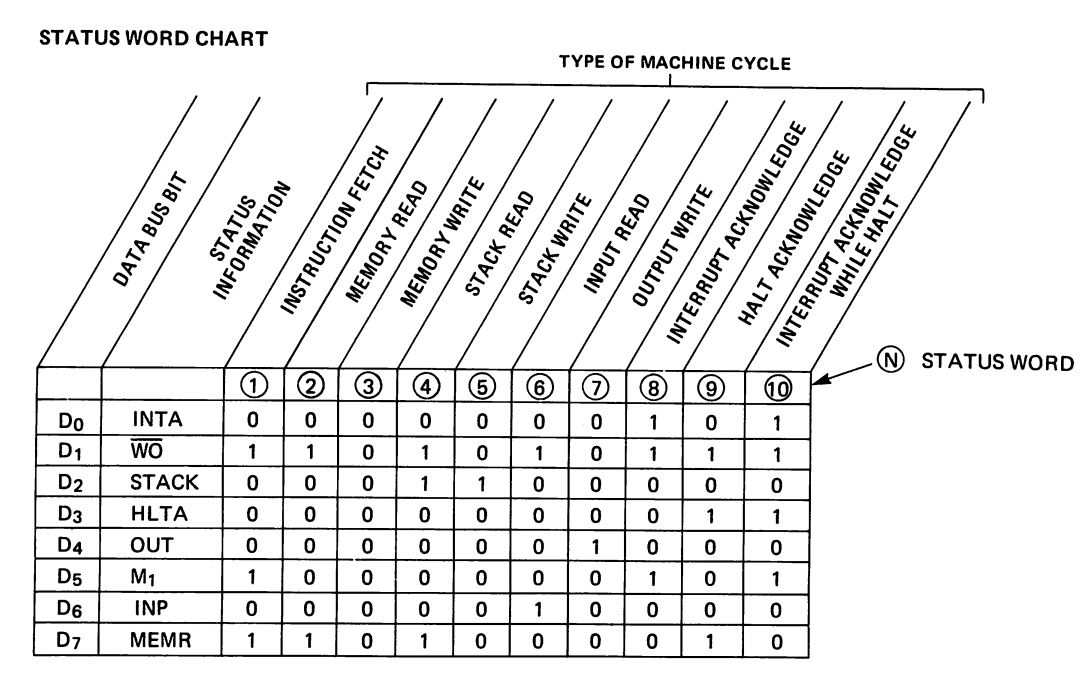
\includegraphics[width=15cm]{Bilder/Intel8080_DataLines}}

\newcommand{\Titel}{Konzeptionierung eines Simulators für 8-bit Prozessoren}
\newcommand{\ArtArbeit}{Studienarbeit}
\newcommand{\Abschluss}{Bachelor of Science}
\newcommand{\Studiengang}{Studiengang Informationstechnik}

\newcommand{\Ort}{Karlsruhe}


\newcommand{\imgSpaceBefore}{\\[0.2cm]}

%\newcommand{\Abgabedatum}{16.02.2021}


\begin{document}
\onehalfspacing
\pagenumbering{Roman}
	\begin{titlepage}
		{\DHBWLogoDeckblatt}\\[2cm]
		\begin{center}
			\vspace*{-2cm}
			{\Huge \Titel}\\[2cm]
			{\Huge \ArtArbeit}\\[2cm]
			{\Large \Abschluss}\\[0.5cm]
			{\large \Studiengang}\\[0.5cm]
			{\large an der}\\[0.5cm]
			{\large Dualen Hochschule Baden-Württemberg Karlsruhe}\\[0.5cm]
			{\large von}\\[0.5cm]
			{\large\bfseries \Autor}\\[1cm]
			{\large Abgabedatum \today}
			\vfill
		\end{center}
		\begin{tabular}{l@{\hspace{1cm}}l}
			Bearbeitungszeitraum & \Bearbeitungszeitraum \\
			Kurs & \Kurs \\
%			Ausbildungsfirma & \Ausbildungsfirma \\
			Betreuer & \Betreuer \\
		\end{tabular}
	\end{titlepage}

\newpage

\thispagestyle{empty}
\begin{center}
\Large\bfseries Erklärung
\end{center}
\medskip
\noindent
Wir versichern hiermit, dass wir unsere \ArtArbeit \ mit
dem Thema: 
\begin{center}
	 \Titel \ 
\end{center}
selbstständig verfasst und keine anderen als die angegebenen Quellen und
Hilfsmittel benutzt haben. Wir versichern zudem, dass die eingereichte elektronische Fassung mit der
gedruckten Fassung übereinstimmt.

\vspace{3cm}
\noindent
\underline{\Ort, \today \hspace{9cm}}\\
%\hfill\underline{\hspace{6cm}}\\
Ort, Datum\hfill Unterschrift\hspace{4cm}

\newpage

\thispagestyle{empty}
\tableofcontents

\newpage

%\thispagestyle{empty}
\thispagestyle{plain}
\cleardoublepage
\addcontentsline{toc}{section}{\listfigurename}
\listoffigures

\addcontentsline{toc}{section}{\listtablename}
\listoftables

\addcontentsline{toc}{section}{Listings}
\lstlistoflistings

\newpage

%\thispagestyle{empty}
\thispagestyle{plain}
\cleardoublepage
\section*{Abkürzungsverzeichnis}
\addcontentsline{toc}{section}{Abkürzungsverzeichnis}
\textbf{ALU} - Arithmetic Logic Unit\\
\textbf{CISC} - Complex Instruction Set Computer\\
\textbf{GUI} - Graphical User Interface\\
\textbf{MISD} - Multiple-instruction stream single-data stream\\
\textbf{MIMD} - Multiple-instruction stream multiple-data stream\\
\textbf{RISC} - Reduced Instruction Set Computer\\
\textbf{SISD} - Single-instruction stream single-data stream\\
\textbf{SIMD} - Single-instruction stream multiple-data stream

\newpage
\pagenumbering{arabic}

%% Kopf und Fusszeilen==================================================== 
\pagestyle{scrheadings} % Seite mit Headern 

% loescht voreingestellte Stile 
\clearpairofpagestyles
%\clearscrheadings 
\clearmainofpairofpagestyles
%\clearscrplain 

% %%% Kopfzeile 
% einseitig: Bei einseitigem Layout, nur folgende Zeilen verwenden !!! 
%\ohead[] {
\includegraphics[height=0.5cm]{Logos/Firmenlogokopfzeile}}
\ihead[]{\leftmark} % links: Kapitel
%\chead[]{} % mitte: 

% %%% Fusszeile 
%\cfoot[]{} % mitte: 
\cfoot[\pagemark]{\pagemark} % rechts: Seitenzahl


% Angezeigte Abschnitte im Header 
\automark{section}  % Inhalt von [\rightmark]{\leftmark} 

\section{Einführung}
Dieses Kapitel befasst sich vorwiegend mit relevanten Grundlagen der Arbeit. Unter anderem wird das Ziel spezifiziert, elementare Aspekte der Arbeitsweise eines Prozessors werden erläutert und die verschiedenen Werkzeuge mit denen das Ziel realisiert wird werden aufgeführt.

\subsection{Ziel der Arbeit}
In dieser Arbeit soll ein Simulationsprogramm geschrieben werden, mit dem mehrere unterschiedliche 8-Bit Prozessoren simuliert werden können. Dazu sollen die Grundlegenden Eigenschaften in kurzen Lernprogrammen erläutert werden. Ebenfalls soll es eine interaktive Einweisung geben wie der Simulator verwendet werden kann.

\subsection{Zeitplan}
Platzhalter

\newpage

\subsection{Theoretische Grundlagen}
Als Vorbereitung für die Implementierung der verschiedenen Prozessoren werden einige allgemeingültige Architekturprinzipien eines Prozessors analysiert. 

\subsubsection{Architektur eines Prozessors}
Der fundamentale Aufbau eines Prozessors lässt sich in folgende Bausteine einteilen:\\
\textbf{Rechenwerk}\\
Das Rechenwerk ist die zentrale Einheit mit der eingehende Befehle verarbeitet werden. Es erhält Werte aus dem Speicher und führt damit in der ALU Operationen durch. Zum Rechenwerk dazugehörig sind auch Hilfsregister die beispielsweise als naher Zwischenspeicher fungieren.\\
\textbf{Steuerwerk}\\
Das Steuerwerk ist für die korrekte Abarbeitung von Befehlen zuständig. Es besteht aus dem Befehlsdekoder, dem Befehlszähler und einem Statusregister.\\
\textbf{Programmspeicher}\\
Der Programmspeicher eines Prozessors enthält die einzelnen Befehle, welche vom Befehlsdekoder dekodiert werden. Dabei wird der Befehl verwendet der an der vom Befehlszähler spezifizierten Stelle im Speicher steht.\\
\textbf{Ein-/Ausgabewerk}\\
Das Ein-/Ausgabewerk ist für die Kommunikation des Prozessors mit anderen Systemkomponenten verantwortlich.\\
\subsubsection{Befehlsformate}
Für einen Prozessor wird zwischen vier verschiedenen Befehlsformaten unterschieden. Diese beziehen sich auf die Anzahl der Adressen, welche der ALU bei Beginn einer Operation zur Verfügung gestellt werden.\\ \\
\textbf{Null-Adress-Anweisungen}\\
Vom Akkumulator (Stack) wird der Wert der zwei obersten Adressfeldern entnommen und die Operation wird auf diese ausgeführt. Der Speicherort des Ergebnisses ist ebenfalls vorbestimmt. Daher werden keine Adressen benötigt zum ausführen von Operationen.\\ \\
\textbf{Ein-Adress-Anweisungen}\\
Wie bei einer Null-Adress-Anweisung wird ein Wert aus dem Akkumulator entnommen. Ein zweiter Wert wird aus dem Speicher der übergebenen Adresse entnommen. Der Speicherort des Ergebnisses ist nach wie vor fest.\\
\textbf{Zwei-Adress-Anweisungen}\\
Für Zwei-Adress-Anweisungen ist es möglich eine Bezugsadresse für die Operanden anzugeben sowie eine Zieladresse, in der das Ergebnis der Operation gespeichert wird.\\ \\
\textbf{Drei-Adress-Anweisungen}\\
Drei-Adress-Anweisungen sind essentiell komplexere Zwei-Adress-Anweisungen. Eine der drei verfügbaren Adressen wird ebenfalls für die Zieladresse der Operation verwendet. Für das Beziehen der Operanden steht eine weitere Adresse zur Verfügung.\\

\subsubsection{CISC und RISC}
Von Andreas
komplettes Kapitel aus Buch \\
Ein Prozessor unterstützt immer nur eine gewisse Menge an Befehlen, diese werden Instruction Set genannt. Heutzutage gibt es zwei grundlegende Prozessorarchitekturen, Complex Instruction Set Computer (CISC) und Reduced Instruction Set Computer (RISC). Früher konnten Prozessoren genau einer dieser Gruppen zugeordnet werden, allerdings ist das bei den heutigen Prozessoren nicht mehr möglich, da sowohl RISC als auch CISC Befehle dem Prozessor zur Verfügung gestellt werden um die Vorteile von beiden zu haben.\\\\
Bei CISC-Prozessoren wird versucht soviel wie möglich in einem Befehl ausführen zu können. So gibt es viele verschieden Befehle, die auch unterschiedlich viel Zeit benötigen. Dadurch wird es aber auch möglich, komplexere Befehle direkt in der Hardware zu berechnen. Bei diesen Befehlen gibt es auch einige Adressierungsarten mehr als bei RISC-Prozessoren. Für vorbestimmte Aufgaben gibt es auch eigene Register, die nur dafür verwendet werden und davon auch nur wenige. Der Nachteil bei CISC-Prozessoren ist, dass die eigenen Befehle erst noch durch ein Mikroprogramm interpretiert werden müssen und dieses die komplexen Befehle in mehrere kleine Befehle aufteilen muss, welche erst dann vom Prozessor bearbeitet werden können. Dies kostet etwas mehr Zeit und verlangsamt die Ausführung. Die Mikroprogramme, die dafür verwendet werden, werden in einem kleinem Read-only Memory (ROM) gespeichert.\\\\
Bei RISC-Prozessoren wird versucht mit nur wenigen, kleinen Befehlen auszukommen. Diese sind wiederum sehr schnell, da sie meist fest verdrahtet sind, müssen aber mit anderen kombiniert werden um die Komplexität eines einzigen CISC-Befehls zu erreichen.  Im Gegensatz zu CISC-Prozessoren besitzen RISC-Prozessoren viele Register die frei verwendbar sind und nicht für speziellen Operationen bestimmt sind. Ebenso können die meisten Befehle in nur einem einzigen Arbeitsschritt ausgeführt werden.\\\\
Da bei CISC-Prozessoren mit nur einem Befehl viel berechnet werden kann, sind diese optimal für Übersetzer oder Interpreter geeignet. Bei der Entwicklung können dann einzelne komplexe Befehle verwendet werden anstatt von vielen kleinen. Jedoch können RISC-Prozessoren schneller Befehle ausführen, da:

\begin{itemize}
\item es nur wenige Befehle gibt und diese schnell decodiert werden können
\item die Befehle mithilfe von Pipelines effizienter abgearbeitet werden können
\item kein Mikroprogramm die einzelnen Befehle erst noch interpretieren muss
\end{itemize}
 

\subsubsection{Parallelität nach Flynn}
Von Andreas\\
1966 wurden von Micheal Flynn die folgenden vier Arten von Parallelisierung eingeführt [Flynn 949]:

\begin{itemize}
\item Single-instruction stream, single-data stream (SISD)
\item Single-instruction stream, multiple-data stream (SIMD)
\item Multiple-instruction stream, single-data stream (MISD)
\item Multiple-instruction stream, multiple-data stream (MIMD)
\end{itemize}
\noindent
\textbf{SISD}\\
Diese Beschreibung trifft auf die einfachen Einprozessorsysteme zu. Dabei kann immer nur eine Operation gleichzeitig ausgeführt werden und diese werden in nur einer möglichen Reihenfolge aus einem Daten-Strom abgearbeitet.\\
\noindent
\textbf{SIMD}\\
Bei SIMD werden Pipelines eingesetzt, die es ermöglichen mehrere korrekte Abfolgen von Programmbefehlen auszuführen. So können unterschiedliche Programme in sich selber in der richtigen Reihenfolge aber mit anderen Programmen abwechselnd ausgeführt werden.\\
\noindent
\textbf{MISD}\\
Diese Variante scheint auf Anhieb keinen effizienten Nutzen zu besitzen, da mehrere Prozessoren alle die gleichen Befehle ausführen, die aus einem Daten-Strom stammen. Dies kann aber dazu verwendet werden um die Korrektheit durch Redundanzen zu bestätigen. \\
\noindent
\textbf{MIMD}\\
Diese Architektur verwendet mehrere Prozessoren und mehrere Daten-Ströme. Heutzutage ist dies unter dem Begriff Mehrprozessorsysteme bekannt. So werden für jeden einzelnen Prozessor ein Daten-Strom erzeugt der unabhängig von den anderen Prozessoren arbeiten kann. Dabei ist es für die Prozessoren aber trotzdem möglich die Daten der anderen Prozessoren zu nutzen. Nur durch MIMD oder MISD, also die Ausführung mit mehreren unabhängigen Prozessoren, ist es möglich Programme tatsächlich parallel ablaufen zu lassen. Mit SISD oder SIMD sind nur quasi parallele Ausführungen möglich.\\

\subsection{Instruction Sets}
Von Andreas\\
Die meisten Prozessoren besitzen Befehle aus den folgenden fünf Gruppen:
\begin{itemize}
\item Daten Transfer Gruppe
\item Arithmetik Gruppe
\item Logische Gruppe
\item Verzweigungs Gruppe
\item Stapel, Ein- Ausgänge und Maschinen Kontroll- Gruppe
\end{itemize}\noindent
Die Befehle der Daten Transfer Gruppe bewegen Daten zwischen Registern und/oder Speicher wie zum Beispiel mit den MOVE Befehlen. In der Arithmetik Gruppe werden, wie der Name schon sagt, Befehle mit arithmetische Operationen wie Addition verwendet. In der Logischen Gruppen werden Operation wie das logische Oder verwendet. In der Zweig Gruppe gibt es die Befehle, welche den Standardmäßigen Programmfluss ändern und das Programm nicht zwangsläufig in der nächsten Zeile fortgesetzt wird wie bei bedingten Sprüngen. In der letzten Gruppe liegen die Befehle, die Eingänge und Ausgänge beachten oder den Stack bearbeiten. [Intel 8080 S.46 (4-1)]
\\

\newpage

\section{Projektplanung}
Bei Projektbeginn wurde kein konkretes Ziel vorgegeben. Es wurde nur verlangt, dass ein Simulator für 8-Bit Prozessoren entwickelt werden soll. Deshalb wurde zu Beginn die Entscheidung getroffen, dass eine kleine Lernsoftware entwickelt werden soll. Der Simulator sollte ursprünglich fähig sein, mehrere unterschiedliche Prozessoren simulieren zu können. Damit sollten die Unterschiede von den einzelnen Prozessoren dargestellt und dem Anwender vermittelt werden. Jedoch hat sich bei der Untersuchung von mehreren Prozessoren herausgestellt, dass es nur geringe Unterschiede zwischen den Prozessoren gibt. Zwar hat jeder Prozessor seine Eigenheiten aber diese sind für den Anwender kaum spürbar. Der größte Unterschied sind die verschiedenen Befehlssätze. Die meisten Prozessoren verwenden für die gleichen Befehle, unterschiedliche Mnemonics und Bitkombinationen. Sobald aber die Befehle decodiert wurden, läuft im Prozessor meistens sehr Ähnliches oder sogar das Gleiche ab. Dabei kann es vorkommen, dass ein Prozessor noch eine zusätzliches Register z.B. als Zwischenspeicher verwendet, welches die anderen nicht besitzen. Aber wie die Daten im Prozessor hin und her geschoben werden und die Befehle, die die ALU ausführt, sind alle sehr ähnlich, wenn nicht sogar identisch. Deshalb wurde sich später dafür entschieden, dass nicht mehrere sondern nur ein Prozessor simuliert werden soll.
\\\\
Bei dem Multi-Prozessor-Simulator war geplant, dass nur die Befehle direkt ausführbar sein sollen. Sodass eine assemblierte Quellcode-Datei eingelesen und ausgeführt werden kann. Diese Implementierung hat nur sicher gestellt, dass die zwangsweise notwendigen Eigenschaften simuliert werden. Dazu zählt, dass die Inhalte von Registern, die vom Anwender verwendet werden können, nach den Befehlen die korrekten Werte enthalten. Zusätzlich dazu wurden auch die Flags simuliert, da diese für den korrekten Programmablauf notwendig sind. 
\\\\
Der Single-Prozessor-Simulator sollte etwas genauer darstellen wie ein Prozessor arbeitet. Dafür wurde der Intel 8080 als Prozessor ausgewählt. Ein Intel 8080 Befehl besteht aus mindestens einem und maximal fünf bzw. in diesem Simulator sechs Maschinen Zyklen. Jeder dieser Maschinen Zyklen besteht wiederum aus mindestens drei und maximal fünf Zuständen. Mit dieser Implementierung kann jeder einzelne Zustand nachvollzogen werden. Dadurch werden auch die W- und Z-Register verwendet, auf die der Anwender normalerweise keinen Zugriff hat und deshalb beim Multi-Prozessor-Simulator nicht beachtet wurden.

\newpage

\subsection{Multi-Prozessor-Simulator}
Mit diesem Simulator soll es möglich sein mehrere unterschiedliche Prozessoren simulieren zu können. Vor der Implementierung des Simulators müssen einer oder mehrere geeignete Prozessoren ausgewählt werden. In den nachfolgenden Kapiteln werden einige potenzielle Kandidaten näher analysiert und beschrieben.



\subsubsection{Z80}
Fällt vermutlich weg

\subsubsection{Beispielprozessor 3 ...}
s.o.\\
Kommentar: Ein weiterer Prozessor sollte zumindest in Ansätzen analysiert werden.

\subsubsection{Intel 8080}
Da der Intel 8080 in dem Single-Prozessor-Simulator verwendet wird und dort auch detaillierter implementiert wird, wird dieser auch dort in Kapitel \ref{SPS}.


\newpage

\subsection{Single-Prozessor-Simulator}
\label{SPS} 
Von Andreas\\ \noindent

Als Prozessor für den Single-Prozessor-Simulator wurde der Intel 8080 ausgewählt. Der Intel8080 bietet ein breites Spektrum an Befehlen und wäre auch repräsentativ für einen der ersten großen, kommerziell erfolgreichen Prozessoren. Aufgrund der überschaubaren Komplexität besteht auch die Möglichkeit diesen in einem größeren Unmfang zu simulieren.

\subsubsection{Register}
\label{RegisterSection}

Der Intel 8080 besitzt ein SRAM Array mit 16-bit Register. Darin enthalten sind der Programm Counter mit 16-bit und der Stack Pointer mit 16-bit. Dazu gibt es noch acht weitere 8-bit Register. Diese können entweder alleine oder zusammen mit einem anderen 8-bit Register als ein 16-bit Register verwendet werden. Dabei gibt es aber nur die fest vorgegebenen Kombinationen. Das B- und C-Register, das D- und E-Register, das H- und L- Register und die temporären W- und Z- Register. Die W- und Z-Register können nicht vom Programmierer verwendet werden und dienen nur zur internen Ausführung von Befehlen. Bei manchen Befehlen wird der Stackpointer als 16-Bit Register verwendet.
Über einen Multiplexer ist es möglich acht Bit auf den internen Adressbus zu schreiben oder von dort zu lesen. \textbf{Über das Adress-Latch oder den Incrementer/Decrementer-Circuit ist es möglich 16-Bit aus den Registern weiterzuleiten. Von dort aus können die Werte dann in den Adress-Puffer geschrieben werden.} [Intel 8080 S16 (2-2)]

\textbf{TODO} Register zuweisung b = 000 etc. einfügen



\begin{figure}[h]
\caption{Kodierung der Register}
\centering
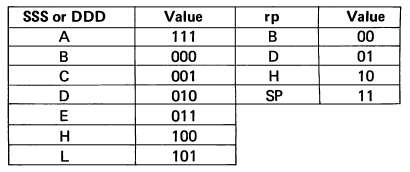
\includegraphics[width=10cm]{Bilder/register_kodierung}
\label{fig:register_kodierung}
\end{figure}

\subsubsection{Befehle}

Der Intel 8080 ist in der Lage Befehle, die aus einem, zwei oder drei Bytes bestehen, auszuführen. Dabei gibt das erste Byte immer den Opcode oder Operation Code an. In Byte zwei und drei werden nur Daten oder Adressen gespeichert. Dabei werden die zwei Byte großen Adressen so gespeichert, dass das niederwertige Byte vor dem höherwertigem gespeichert wird. Die Adressen können dabei über vier verschiedene Modi verwendet werden.
\begin{itemize}
\item Direct
\item Register
\item Register Indirect
\item Immediate
\end{itemize}\noindent
Bei "Direkt"' wird der Wert in dem Speicher mit der angegebenen Adresse verwendet. Hier werden das Low-Byte im zweiten und das High-Byte im dritten Byte gespeichert. Bei "Register"' wird auf ein oder zwei Register verwiesen und verhält sich wie bei Direkt. Bei "Register Indirect"' wird der Wert aus der Adresse aus dem zweiten und dritten Byte des Befehls gelesen. Dieser Wert wird als Adresse verarbeitet und erst der Wert aus dieser Adresse ist der zu verwendete Wert. Bei [TODO]\glqq Immediate\grqq steht 
im zweiten und/oder dritten Byte ein Wert mit dem gearbeitet wird (Lowbyte im zweiten Byte). [Intel 8080 S.47 (4-2)]
\\ \noindent
Bei Interrupts und Branch Befehlen gibt es nur den "Direct"' und "Register indirect"' Modus [Intel 8080 S.47 (4-2)]. 
\\ \noindent
Der Prozessor besitzt fünf Condition Flags. Das Zero flag, das angibt ob das Ergebnis eines Befehls den Wert 0 hatte. Das Sign flag, welches angibt ob Bit 8, das Most Signifikant-Bit, des letzten Ergebnisses den Wert 1 hat. Das Paritäts flag, welches gesetzt ist, wenn das letzte Ergebnis einen Modulo 2 Wert von 0 hat, also der Wert gerade ist. Das Carry flag, das einen Übertrag bei einer Addition oder einen Abzug bei einer Subtraktion oder Vergleich anzeigt und noch das Auxiliary Carry flag, welches ebenfalls einen Übertrag oder Abzug anzeigt aber zwischen dem vierten (Bit 3) und fünften Bit (Bit 4). [Intel 8080 S.47f (4-2)]
\\

\subsubsection{OP-Code Codierung}
\label{chapter:opcode}
Jedem Befehl ist ein Byte (OP-Code) zugewiesen. Dabei gibt es mehrere Typen. In manchen Befehlen werden einzelne Bits verwendet um Register oder Registerpaare zu codieren und andere bei denen jedes Bit verwendet wird. In \ref{table:opcode} stehen die verschiedenen Möglichkeiten. Bei dem Befehl ACI ist es wichtig, dass das Byte genau 0xC7 ist. Bei ADC und INR wird ein 8-Bit Register in den Befehl codiert. Hierbei wird unterschieden, ob Daten in das Register geschrieben (DDD für Destination) oder daraus gelesen (SSS für Source) werden. Bei Mov r1, r2 wird sowohl aus einem Register gelesen als auch in ein anderes geschrieben, weshalb nur noch zwei Bit für den eigentlichen MOV-Befehl übrig bleiben. Bei dem INX-Befehl wird ein 16-Bit Register verwendet. Wie auf Seite \pageref{RegisterSection} beschrieben, können auch zwei 8-Bit-Register zu einem 16-Bit-Register zusammen geschlossen werden und damit verwendet werden. Insgesamt gibt es davon drei Kombinationen. Dementsprechend werden in diesen Befehlen diese Register mit zwei Bit kodiert. Damit gibt es noch eine weitere Bitkombination, mit der ein weiteres Register verwendet werden kann. Mit der vierten noch übrig gebliebenen Kombination wird der Stackpointer als 16-Bit-Register verwendet werden. 

\begin{table}[h]
\centering
\caption{Op-Code Typen}
\label{table:opcode}
\begin{tabular}{|l|c|c|c| } 
 \hline
 Befehl & OP-Code \\
 \hline 
 ACI & \texttt{1100 1110} \\ 
 ADC r & \texttt{1000 1SSS} \\
 INR r & \texttt{00DD D101} \\
 MOV r1, r2 & \texttt{01DD DSSS} \\
 INX rp & \texttt{00RP 0011} \\
 \hline
\end{tabular}
\end{table}

\subsubsection{Data Transfer Group}
Für den Prozessor sind 13 Befehle aus dieser Gruppe bekannt. Bei keinem dieser Befehle werden die Condition Flags gesetzt oder zurückgesetzt.

\begin{multicols}{2}
\begin{itemize}
\item Move Register
\item Move from Memory
\item Move to Memory
\item Move immediate
\item Move to Memory Immediate
\item Load register pair immediate
\item Load Accumulator direct
\item Store Accumulator direct
\item Load H and L direct
\item Store H and L direct
\item Load Acumulator indirect
\item Store Accumulator indirect
\item Exchange H and L with D and E
\end{itemize}
\end{multicols}


\subsubsection{Arithmetic Group}
20 Befehle
Unless indicated otherwise, all instructions in this
group affect the Zero, Sign, Parity, Carry, and Auxiliary
Carry flags accord ing to the standard rules.
All subtraction operations are performed via two's
complement arithmetic and set the carry flag to one to indicate a borrow and clear it to indicate no borrow

\begin{multicols}{2}
\begin{itemize}
\item Add Register
\item Add Memory
\item Add immediate
\item Add Register with carry
\item Add Memory with carry
\item Add immediate with carry
\item Sustract Register
\item Subtract Memory
\item Subtract immediate
\item Subtract Register with borrow
\item Subtract Memory with borrow
\item Subtract immediate with borrow
\item Increment Register
\item Increment Memory
\item Decrement Register
\item Decrement Memory
\item Increment register pair
\item Decrement register pair
\item Add register pair to H and L
\item Decimal Adjust Accumulator
\end{itemize}
\end{multicols}

\subsubsection{Logical Group}
19 Befehle
Unless indicated otherwise, all instructions in this
group affect the Zero, Sign, Parity, Auxiliary Carry, and
Carry flags according to the standard rules

\begin{multicols}{2}
\begin{itemize}
\item AND Register
\item AND Memory
\item AND immediate
\item Exclusive OR Register
\item Exclusive OR Memory
\item Exclusive OR immediate
\item OR Register
\item OR Memory
\item OR immediate
\item Compare Register
\item Compare Memory
\item Compare immediate
\item Rotate left
\item Rotate right
\item Rotate left through Carry
\item Rotate right through Carry
\item Complement Accumulator
\item Complement Carry
\item Set Carry
\end{itemize}
\end{multicols}


\subsubsection{Branch Group}
8 Befehle
Flags are not affected

\begin{itemize}
\item Jump
\item Conditional Jump
\item Call
\item Conditional Call
\item Return
\item Conditional Return
\item Restart
\item Jump H and L indirect - move H and L to PC
\end{itemize}

\subsubsection{Stack, I/O and Machine Control Group}
12  Befehle
Unless otherwise specified, condition flags are not
affected by any instructions in this group

\begin{multicols}{2}
\begin{itemize}
\item Push
\item Push Processor status word
\item Pop
\item Pop processor status word
\item Exchange stack top with H and L
\item Move HL to SP
\item Input
\item Output
\item Enable Interrupts
\item Disable Interrupts
\item Halt
\item No op
\end{itemize}
\end{multicols}


\subsubsection{Maschinenzyklen und Typen}
Jeder Befehl oder Befehlszyklus benötigt mindestens einen und maximal fünf Maschinenzyklen zum kompletten Ausführen des Befehls. Dabei kann jeder Befehl aus mehreren Typen bestehen, wobei der erste immer ein Fetch-Befehlstyp ist. Die existierenden Befehlstypen sind:

\begin{itemize}
\item Fetch
\item Memory Read
\item Memory Write
\item Stack Read
\item Stack Write
\item Input
\item Output
\item Interrupt
\item Halt
\item Halt Interrupt
\end{itemize}\noindent
Jeder Maschinenzyklus besteht nochmal aus drei bis fünf Zuständen. So kann ein Befehl insgesamt zwischen vier und achtzehn Zuständen andauern.
In dem ersten Zustand jedes Maschinenzykluses wird immer der Befehlstyp während des SYNC-Taktes kodiert. Die folgende Abbildung zeigt, wie die Befehlstypen über die \textbf{Data Lines} kodiert werden. [Intel 8080 S17ff. 2-3]
\imgSpaceBefore


\newpage

\section{Umsetzung}
In diesem Kapitel wird darauf eingegangen wie die in Kapitel 2 erarbeitete Analyse der ausgewählten Prozessoren implementiert wird.

\subsection{Abstraktion der Architektur}
Es ist vorgesehen, dass der Prozessor in verschiedene Unterklassen aufgeteilt wird. Dabei ist vorgesehen das dies in einer Art Stern-Struktur aufgebaut wird, das heißt die verschiedenen Bestandteile des Prozessors sollen alle mit einer zentralen Klasse interagieren, aber nicht untereinander.

\subsubsection{Prozessor}
Die Prozessor-Klasse soll die zentrale Einheit des Simulators sein. Über diese sollen sowohl Anfragen über Informationen vorgenommen werden, zum Beispiel um diese in der Benutzeroberfläche anzuzeigen, als auch Instruktionen an den Prozessor als ganzes gesendet werden. Dabei ist zu unterscheiden zwischen zwei Arten von Anfragen, gültige und ungültige. Gemeint ist sind damit Anfragen in einem echten Prozessor zulässig wären, beispielsweise einen externen Bus zu befüllen oder die nächste Anweisung auszuführen, und Anfragen die unzulässig wären, wie den Programmzähler manuell zu setzen.

\subsubsection{ALU}
Die ALU soll die Bearbeitung logischer Operationen im Prozessor simulieren. Sinn ist dabei ein möglichst genaues Bild jedes Zustandes des Prozessors darzustellen, statt beispielsweise solche Operationen einfach manuell in der Prozessor-Klasse abzuarbeiten.

\subsubsection{Register}
Die Register-Klasse soll ähnlich wie die ALU den Zugriff möglichst realitätsgetreu simulieren. Dabei sollen Methoden die den Zugriff regeln ähnlich aufgebaut werden wie es im echten Prozessor möglich wäre.

\subsubsection{Peripherie}
Mit der Peripherie soll alles abgedeckt werden was nicht Teil der zentralen Bestandteile ist, also der Register oder der ALU. Dazu zählt zum Beispiel ein externer Datenbus oder Schnittstellen für bspw. Taktsignal o.ä.

\subsection{Möglichkeiten der Simulation}
Um einen Ablauf für die Simulation festzulegen muss erst bestimmt welche Parameter eingestellt, welche Optionen verändert und welche Operationen im Simulator durchgeführt werden können.

\subsection{Ablauf der Simulation}
Platzhalter

\subsection{Aufbau der GUI}
\label{chp:AufbauGUI}
Das Simulieren des Prozessors ist die eine Seite dieses Projekts. Gleichermaßen wichtig für einen funktionierenden Simulator ist aber auch die Benutzeroberfläche mit der dieser bedient wird. In diesem Abschnitts werden die einzelnen Aspekte dieser analysiert.
\subsubsection{Hauptmenü}
Bei Programmstart wird das in Abbildung \ref{fig:Hauptmenue} gezeigte Fenster geöffnet.

\begin{figure}[h]
\centering
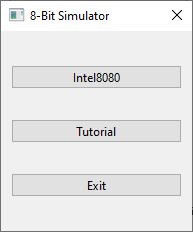
\includegraphics[width=6cm]{bilder/Hauptmenue}
\caption{Hauptmenü}
\label{fig:Hauptmenue}
\end{figure}

\noindent
Die Aufgabe dieses Fensters ist simpel. Es gibt 3 verschiedene Knöpfe die jeweils eine Funktion erfüllen.
\begin{itemize}
	\item Intel8080: Öffnet das Simulationsfenster des Intel8080 Prozessors
	\item Tutorial: Öffnet ein Fenster welches eine kurze Einweisung gibt in die Handhabung des Simulators für den Intel8080
	\item Exit: Schließt das Fenster und alle laufenden Hintergrundprozesse, für den Fall das ein Simulatorprozess in der selben Session verwendet wurde.
\end{itemize}

\subsubsection{Intel8080 Simulationsfenster}
In Abbildung \ref{fig:I8080MW} ist die aktuellste Version des Simulationsfensters für den Intel8080 zu sehen.

\begin{figure}[h]
\centering
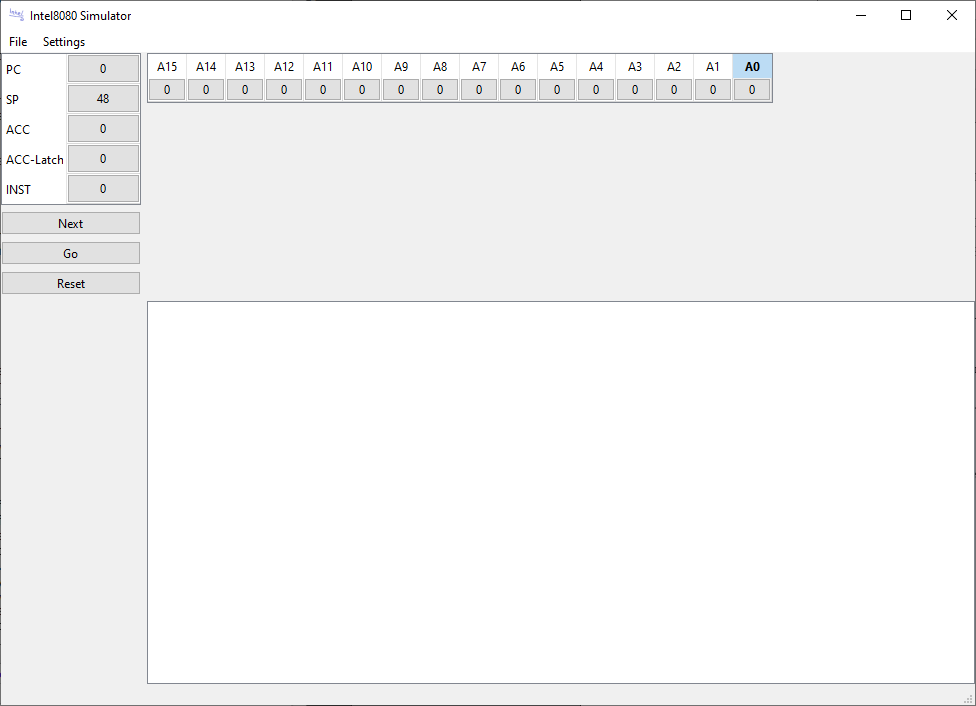
\includegraphics[width=15cm]{bilder/Intel8080_MainWindow}
\caption{Intel8080 Sumulationsfenster}
\label{fig:I8080MW}
\end{figure}

\noindent
Über das Simulationsfenster für den Intel8080 können Programme die aus Bytebefehlen bestehen, welche ein Intel8080 Prozessor ausführen kann, simuliert werden. Dafür muss sollte (muss aber nicht) zuerst ein gültiges Programm geladen werden. Dies kann über den Reiter 'File' in der Menüleiste getan werden (siehe Abbildung \ref{fig:LoadFile}).

\begin{figure}[h]
\centering
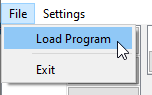
\includegraphics[width=6cm]{bilder/LoadFile}
\caption{File Reiter}
\label{fig:LoadFile}
\end{figure}

\noindent
Dadurch öffnet sich ein Dateien-Explorer über den die gewünschte Datei ausgewählt werden kann. Dabei ist zu beachten, dass in der aktuellen Version nur Ausgabedateien des verwendeten Assemblers genutzt werden können (Dateiendung '.com'). Abgesehen davon kann über 'Exit' auch ins Hauptmenü zurückgekehrt werden. Sobald ein Programm geladen wurde, wird dieses in der dafür vorgesehenen Tabelle angezeigt (siehe Abbildung \ref{fig:ProgTable}).

\begin{figure}[h]
\centering
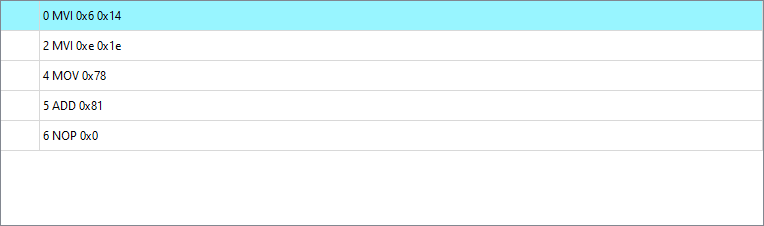
\includegraphics[width=15cm]{bilder/Program_table}
\caption{Programm Tabelle}
\label{fig:ProgTable}
\end{figure}

\noindent
Dabei ist für jeden Befehl eine Zeile vorgesehen. Angezeigt wird einerseits die Position des Bytebefehls im Speicher, die Bezeichnung des Befehls, der Bytecode selbst als auch zusätzliche Parameter falls der jeweilige Befehl welche besitzt. Außerdem wird die Zeile die als nächstes ausgeführt wird farbig markiert. Abgesehen von der Anzeige des Programms und des als nächstes ausgeführten Befehls ist es auch möglich Breakpoints zu setzen (siehe \ref{fig:Break}).

\begin{figure}[h]
\centering
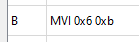
\includegraphics[width=6cm]{bilder/Breakpoint}
\caption{Breakpoint}
\label{fig:Break}
\end{figure}

\noindent
Diese sind relevant wenn das Programm automatisch ausgeführt wird (siehe nächster Abschnitt). Wird ein Breakpoint erreicht, so stoppt das Programm bevor der Befehl ausgeführt wird und das Programm muss entweder manuell oder erneut automatisch ausgeführt werden. Da vorgesehen ist, dass das gesamte Programm in dieser Tabelle angezeigt wird, ist eine Sonderbehandlung des NOP-Befehls notwendig. Dieser wird durch den Bytecode '0x00' identifiziert. Bei initialisieren des Speichers ist dies auch die Standardbelegung jedes Registers. Damit die Tabelle also nicht mit in den meisten Fällen unnötigen NOP-Befehlen befüllt wird, musste dafür eine Ausnahmeregelung getroffen werden. Sind im Speicher zwei oder mehr NOP-Befehle direkt aufeinanderfolgend, werden diese zu einem Eintrag zusammengefasst. Da diese Tabelle lediglich das Programm in komprimierter Weise darstellt aber keine Interaktion mit diesem ermöglicht würde zusätzlich das in Abbildung \ref{fig:ProgSpeicher} gezeigte Fenster in die GUI eingefügt.

\begin{figure}[h]
\centering
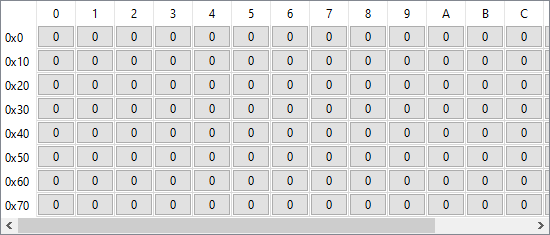
\includegraphics[width=12cm]{bilder/ProgramMemory}
\caption{Programmspeicher}
\label{fig:ProgSpeicher}
\end{figure}

\noindent
Dieses ermöglicht es den Speicher separat vom Programm auszulesen in Abschnitten von 128 Registern, wobei pro Zeile jeweils sechzehn Register, eins pro Spalte, zu sehen sind. Hierbei ist es im Gegensatz zur oben beschriebenen Tabelle möglich diese zu bearbeiten. Dies geschieht durch klicken der entsprechenden Zelle, wodurch sich ein Dialog öffnet. Änderungen werden bei der nächsten Zustandsänderung ('Next State/Machine Cycle/Instruction') in die Programmtabelle übernommen. Um auszuwählen, welche Register aus dem Programmspeicher angezeigt werden, kann das in Abbildung \ref{fig:Range} gezeigte Interface, verwendet werden.

\begin{figure}[h]
\centering
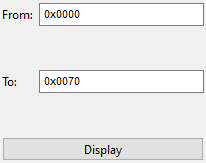
\includegraphics[width=6cm]{bilder/Range}
\caption{Range Einstellungen}
\label{fig:Range}
\end{figure}

\noindent
Hierbei kann entweder eingestellt werden bis zu oder ab welchem Register der Speicher angezeigt werden soll. Wird einer der beiden Werte verändert ergänzt sich der andere automatisch. Der Abstand muss dabei immer genau 128 Register sein. Eingetragene Werte müssen außerdem immer ein Vielfaches von sechzehn sein, da dies der Anzahl an Registern einer Zeile entspricht. Um das Programm auszuführen werden fünf Knöpfe verwendet (siehe Abbildung \ref{fig:Bedienen}).
\newpage

\begin{figure}[h]
\centering
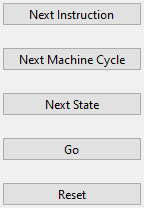
\includegraphics[width=6cm]{bilder/Bedienen}
\caption{Bedien-Knöpfe}
\label{fig:Bedienen}
\end{figure}

\noindent
Über 'Next Instruction' wird der nächste Befehl, also der in der Programm Tabelle farbig markierte, ausgeführt und die Benutzeroberfläche wird entsprechend aktualisiert. Dasselbe gilt für 'Next Machine Cycle' als auch für 'Next State', wobei diese wiederum nur den nächsten Machinenzyklus oder den nächsten Zustand ausführen. Über Go wird automatisch das Programm ausgeführt. Bei erneutem drücken wird das Programm pausiert. Reset setzt den Simulator auf die Ausgangssituation zurück, behält aber den aktuellen Zustand des Programmspeichers bei. Es ist auch möglich einzelne Register des Prozessors auszulesen. Wie in Abbildung \ref{fig:Register} zu sehen sind diese mit deren entsprechender Bedeutung gekennzeichnet sowie deren Wert daneben.

\begin{figure}[h]
\centering
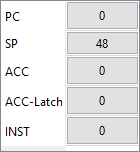
\includegraphics[width=4cm]{bilder/Register}
\caption{Ausgewählte besondere Register}
\label{fig:Register}
\end{figure}

\noindent
Die gezeigten Einträge stehen für:

\begin{itemize}
	\item PC: Program Counter Register
	\item SP: Stack Pointer Register
	\item ACC: Accumulator Register
	\item ACC-Latch: Accumulator-Latch Register
	\item INST: Instruction Register
\end{itemize}

\noindent
Über die Knöpfe daneben in denen die entsprechenden Werte stehen lässt sich über klicken dieser ein Fenster öffnen, welches erlaubt den Wert zu ändern.
Das in Abbildung \ref{fig:GenReg} gezeigte Fenster ist für die restlichen Register zuständig.

\begin{figure}[h]
\centering
\begin{subfigure}{.5\textwidth}
  \centering
  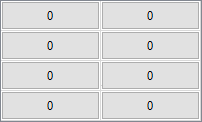
\includegraphics[width=.7\linewidth]{bilder/GenericRegister_sim}
  \caption{Simualtor generische Register}
  \label{fig:GenReg_s}
\end{subfigure}%
\begin{subfigure}{.5\textwidth}
  \centering
  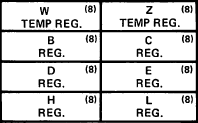
\includegraphics[width=.7\linewidth]{bilder/GenericRegister_pic}
  \caption{Äquivalente Darstellung}
  \label{fig:GenReg_p}
\end{subfigure}
\caption{Simulator Register und Darstellung}
\label{fig:GenReg}
\end{figure}

\noindent
Damit gemeint sind die generischen Register ohne feste Funktion, welche jeweils eine Speicherkapazität von acht Bit haben. Über die in Abbildung \ref{fig:Interrupt} dargestellte Funktion ist es möglich ein Interrupt mit einem gültigen Interrupt-Bytevektor auszulösen.

\begin{figure}[h]
\centering
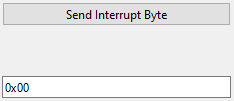
\includegraphics[width=6cm]{bilder/Interrupt}
\caption{Interrupt Byte senden}
\label{fig:Interrupt}
\end{figure}

\noindent
Dabei wird geprüft ob die Operation gültig ist, wenn nicht wird eine Fehlermeldung ausgegeben. Ist sie gültig wird sie beim nächstmöglichen Zustand berücksichtigt und ausgeführt.
\newpage
\noindent
Die letzte Funktionalität der Benutzeroberfläche ist ein Log in dem die einzelnen Operationen aufgelistet werden die in jedem State vorgenommen werden (siehe Abbildung \ref{fig:Logger}).

\begin{figure}[h]
\centering
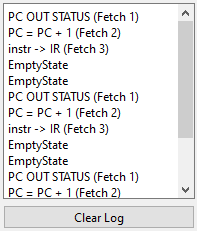
\includegraphics[width=6cm]{bilder/Logger}
\caption{State Log für aufeinanderfolgende NOP-Befehle}
\label{fig:Logger}
\end{figure}

\noindent
Ein nicht mehr in der finalen Version der GUI vorhandenes Register, welches dem Nutzer angezeigt wird und welches bearbeitet werden kann ist in Abbildung \ref{fig:AddBuff} zu sehen.

\begin{figure}[h]
\centering
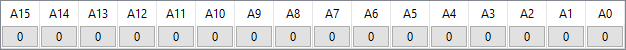
\includegraphics[width=15cm]{bilder/AddBuff}
\caption{Adresspuffer}
\label{fig:AddBuff}
\end{figure}

\noindent
Gezeigt ist der Adresspuffer, welcher für das Auswählen von externen Geräten über das Bussystem zuständig ist. Die Darstellung wurde hier bitweise gewählt, das heißt, statt die ganzen 2 Byte des Registers zu bearbeiten, steuert man die Bits einzeln an.

\subsection{Tutorial}

\newpage

\section{Implementierung}
Von Andreas
\\
\noindent
In diesem Kapitel wird gezeigt, was programmiert wurde, bis sich entschlossen wurde nur einen Prozessor zu simulieren. Obwohl dieser Simulator eigentlich mehrere Prozessoren simulieren können sollte, konnte dieser nie mehr als den Intel 8080 simulieren. Bei der Vorbereitung einen neuen Prozessor zu simulieren, ist aufgefallen, dass die Prozessoren sich nur minimal Unterscheiden werden. Mit dieser Erkenntnis wurde dann der bisherige Simulator so umgebaut, dass ein Prozessor detaillierter simuliert wird. Dessen Implementierung wurde in Kapitel \ref{SPS_impl} beschrieben.


\subsection{Multi-Prozessor-Simulator}
Mit diesem Simulator soll es möglich sein Assembler Code in ein Textfeld einzugeben und diesen dann ausführen zu können. Damit dies möglich ist muss der Assembler Code erst erstellt werden. Dies wird mit einem einfachen Assembler aus dem Internet gemacht. Dieser erstellt aus dem Source Code (.asm) eine .com-Datei, woraus die Befehle byteweise ausgelesen werden können. Manche Befehle verwenden aber auch mehr als ein Byte. Zusätzlich dazu wird noch eine Datei (.sym) erstellt, die die Lables/Sprungmarken abspeichert.
\noindent


\subsubsection{Programmablauf}
Der eigentliche Simulator verwendet nur die .com-Dateien. Als aller erstes wird die .com-Datei ausgelesen und in den Programmspeicher des Prozessors geschrieben. Um den ersten Befehl ausführen zu können wird zuerst nur ein Byte aus dem Programmspeicher, an der Stelle des Programmzählers, eingelesen. Danach wird das erste Byte dekodiert. 
Je nach Befehl werden noch weitere Bytes eingelesen, die für den eigentlichen Befehl benötigt werden. Sobald alle nötigen Informationen eingelesen wurden, wird der Befehl ausgeführt. Jeder Befehl muss entsprechend den Programmzähler anpassen, damit der nächste Befehl wieder korrekt eingelesen werden kann. Mit diesem Simulator ist es auch möglich Interrupts auszulösen. Vor jedem Befehl wird geschaut, ob ein Interrupt ausgelöst wurde. Falls das der Fall ist, wird das Interrupt-Byte ausgewertet und ausgeführt. Normalerweise wird dieses Byte von dem Interrupt Erzeuger mitgeschickt. Meistens ist dies ein Reset-Befehl, der an eine von acht Stellen springt und die dort liegenden Befehle ausführt. Mit 3 Bits kann damit entschieden werden wo die Subroutine beginnen soll. Byte 0, 8, 16 ... 56. Es ist aber auch möglich, dass ein anderer, ein Byte Befehl übergeben, und direkt ausgeführt wird. Während des Interrupts werden weitere Interrupts ignoriert außer in der Interrupt Service Routine werden Interrupts explizit wieder aktiviert.


\subsubsection{Dekodieren eines Befehls}
\noindent
Um aus einem Byte ein Befehl analysieren zu können, wird dieser Wert mehrfach mit vielen Hexadezimalen Werten verglichen. Anhand der Dokumentation des Intel 8080 werden somit alle Befehle unterschieden. 
\textbf{[TODO]} Wie in  Abbildung \ref{fig:ReadInstruction} zu sehen ist, wird der Befehl \glqq Add Immediate to A with carry (ACI)\grqq mit dem Wert 0xCE assoziiert.  
Bei vielen Befehlen wie ACI wird auf genau einen Wert geprüft. Es gibt aber auch andere Befehle, wobei nicht alle Bits des Bytes den Befehl beschreiben. In Abbildung \ref{fig:ReadInstruction} ist zu sehen, dass der Befehl \glqq Add Memory to A with carry (ADC)\grqq nicht so einfach verglichen wird. Bei diesem Befehl werden in den letzten drei Bits des Befehlsbytes das 8-Bit-Register kodiert, welches verwendet werden soll. Deshalb wird die Instruction Variable zuerst mit dem Wert 0xF8 bitweise verundet, damit die letzten drei Bit ignoriert werden. Somit werden alle Bitkombinationen erkannt, bei denen die ersten fünf Bits mit dem Wert 0x88 übereinstimmen. Wenn dann bekannt ist, dass es sich um einen ADC-Befehl handelt, wird das Register ermittelt, das verwendet werden soll. Dies geschieht über die get\_reg8d\_from\_inst(instruction)-Methode. Für die unterschiedlichen Fälle, der Register-Kodierung, gibt es jeweils eine eigene Methode. Diese liefert einen Wert zwischen Null und Acht. Entsprechend der Abbildung \ref{fig:register_kodierung}.
\imgSpaceBefore
\begin{figure}[h]
\caption{Lesen und dekodieren eines Bytes}
\centering
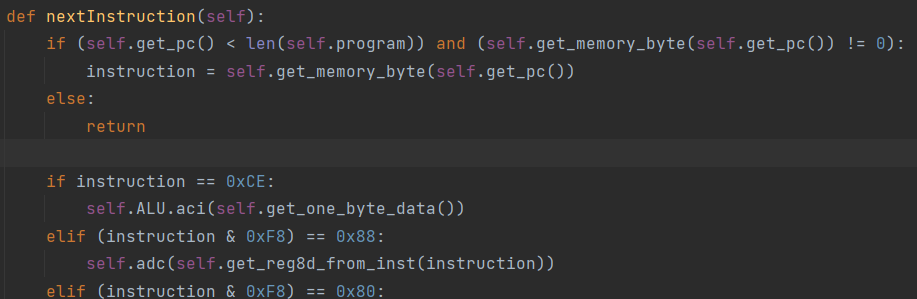
\includegraphics[width=10cm]{Bilder/ReadInstruction}
\label{fig:ReadInstruction}
\end{figure}

\noindent
Dieses Vorgehen wird bei einigen Befehlen verwendet. In Kapitel \ref{chapter:opcode} wird genauer gezeigt, wie die Register in den Befehlen codiert werden.


\subsubsection{Programmaufbau}
\label{chapter:MPS_aufbau}

Der Simulator besteht hauptsächlich aus drei Klassen:

\begin{itemize}
\item Dem Prozessor (Intel8080.py)
\item Der ALU (Intel8080\_ALU.py)
\item Die Register (Intel8080\_Registers.py)
\end{itemize} 

Die Register-Klasse ist hauptsächlich als Datenspeicher gedacht und besitzt keine spezielle Methoden. In der Prozessor- und der ALU-Klasse werden Befehle ausgeführt. Es werden zwei Arten von Befehlen unterschieden. Befehle wie Sprungbefehle, die die ALU nicht benötigen und Befehle wie Additionen, die die ALU verwenden. 
Die Befehle, die die ALU nicht verwenden wurden in in der Intel8080.py implementiert. Die restlichen entsprechend in der ALU. Jeder Befehl wird durch eine eigene Methode implementiert. Somit kann ein Befehl schnell gefunden und angepasst werden. In diesen Methoden läuft der komplette Befehl ab. Somit werden in diesen Methoden auch weitere Bytes eingelesen, die für die Ausführung des Befehls notwendig sind.
Bei jedem Lesevorgang aus dem Programmspeicher (nur wenn die entsprechende Methode verwendet wird) wird der Programmzähler automatisch um eins erhöht. Damit ist es nicht möglich das gleiche Byte mehrfach hintereinander zu lesen. Um das gleiche Byte nochmal lesen zu können, müsste der Programmzähler manuell angepasst werden.
\imgSpaceBefore
\begin{figure}[h]
\caption{Implementierung des Lesens eines Bytes}
\centering
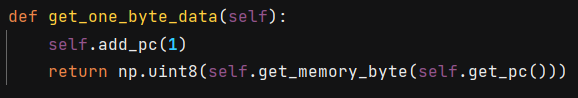
\includegraphics[width=15cm]{Bilder/GetOneByteData}
\label{fig:GetOneByteData}
\end{figure}

\noindent
Der Befehl DCX reduziert das angegebene 16-Bit Register um 1. 
Abbildung \ref{fig:dcx_impl} zeigt die Implementierung des DCX Befehls. 
Dort ist zu sehen, dass es bei den 16-Bit Registern ein grundlegende Unterscheidung gibt. Es gibt einen Fall für den Stackpointer und einen für die anderen 16-Bit Register, die aus zwei 8-Bit Registern zusammengesetzt werden. Mittels des Übergebenen Parameter rp kann ermittelt werden ob es sich um den Stackpointer (rp  == 3 bedeutet Stackpointer) handelt, der angepasst werden soll. 
Der Stackpointer kann einfach einmal ausgelesen, um 1 reduziert und dann wieder in sein Register gespeichert werden.
Bei den zusammengesetzten 16-Bit Registern, werden zuerst beide 8-Bit Register ausgelesen und dann zusammengebaut. Dieses Ergebnis kann dann um 1 reduziert werden. Danach wird der 16-Bit Wert wieder aufgetrennt und in die 8-Bit Register gespeichert. 
\imgSpaceBefore
\begin{figure}[H]
\caption{Implementierung des DCX-Befehls}
\centering
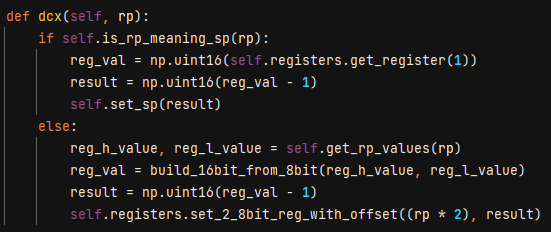
\includegraphics[width=15cm]{Bilder/dcx_impl}
\label{fig:dcx_impl}
\end{figure}

\noindent
Die zusammengesetzten Register können alle gleich behandelt werden, da bei dem Programmkonzept daran gedacht wurde, dass dies öfter vorkommen kann. Deshalb wurden die Register so positioniert, dass auf die Register anhand ihrer Kodierung (siehe. \ref{fig:register_kodierung}) direkt zugegriffen werden kann. Ebenso liegt damit das High Byte eines 16-Bit Registers einen Platz vor dem Low Byte. Mit dieser Anordnung kann mittels einfacher mathematischer Berechnungen die entsprechenden Array-Stelle ermittelt werden. So kann aus einem rp-Wert (0-2) das entsprechende Array-Feld (High Byte) mittels einer Multiplikation mit 2 und der Addition eines Offsets berechnet werden. Um auf das Low Byte zu kommen, muss dann nur noch 1 addiert werden.
\imgSpaceBefore
\begin{figure}[H]
\caption{Register Array des Intel8080}
\centering
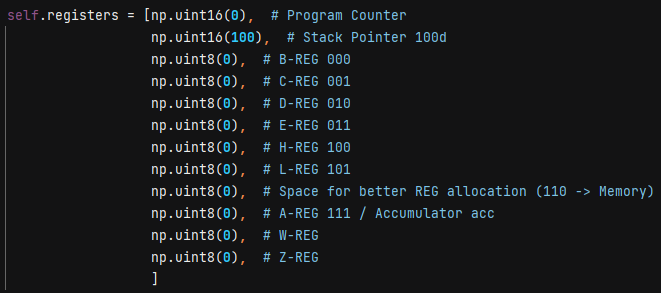
\includegraphics[width=15cm]{Bilder/register_array}
\label{fig:reg_array}
\end{figure}


\noindent


\subsubsection{Befehlsvarianten}

Der Intel 8080 kennt mehrere Befehle, die sowohl eine direkte als auch eine indirekte Variante besitzen. Der Unterschied ist nur, dass die Werte, mit denen gerechnet wird, von unterschiedliche Stellen geladen werden. Aus diesem Grund greifen beide Befehle im Hintergrund auf die gleichen Methoden zu. Somit ist sicher gestellt, dass falls etwas an der Implementierung geändert werden soll, das nur an einer Stelle gemacht werden muss.
\\
Ein Beispiel dafür ist die \glqq Subtract register/immediate from A with borrow (SBB/SBI)\grqq. Es gibt für beide Mnemonics eine Methode in der Intel8080-Klasse aber die Methode von SBB leitet später in der ALU-Klasse nur noch auf die SBI-Methode weiter.
\imgSpaceBefore
\begin{figure}[h]
\caption{Zugrunde liegende Implementierung von SBB und SBI}
\centering
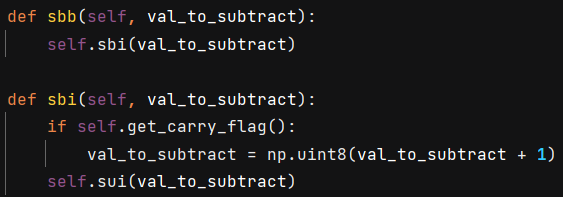
\includegraphics[width=15cm]{Bilder/DoubleUsedMethodSubtract}
\label{fig:DoubleUsedMethodSubtract}
\end{figure}

\noindent
Die direkten Befehle lesen das zweite Byte, das zu diesem Befehl gehört und rufen die
Methode SBI in der ALU-Klasse auf. Für indirekte Befehle wie SBB wird zuerst in der Intel8080-Klasse noch der Wert aus dem Speicher gelesen. Dies wird deshalb gemacht, da die ALU eigentlich keinen direkten Zugriff auf den Speicher hat. Mit dem gelesenem Wert wird dann in der ALU-Klasse die SBB-Methode aufgerufen. Diese leitet innerhalb der Klasse nur noch auf die SBI Methode weiter.
\\\\
Ähnliches wird auch bei bei den Sprungbefehlen gemacht. Dort gibt es mehrere Varianten, die aber nur auf unterschiedliche Flags reagieren. Deshalb wurde auch dort eine zugrundeliegende Methode geschrieben, auf die alle anderen verweisen. So wird nur für die spezifische Varianten, das verwendete Flag weitergegeben.  Abbildung \ref{fig:JumpVariants} zeigt wie bei dem Jump on Carry Befehl vorgegangen wird. So ruft die jc-Methode, die jump\-on-Methode mit dem Carry-Flag auf. In der jump\_on-Methode werden immer die nächsten zwei Bytes gelesen, die die Adresse beinhaltet, auf die gesprungen werden soll. Nur sofern das übergebene Flag gesetzt ist wird der Sprung ausgeführt. Wenn nicht wird das Programm normal weitergeführt.
\imgSpaceBefore
\begin{figure}[H]
\caption{Implementierung der Sprungbefehle}
\centering
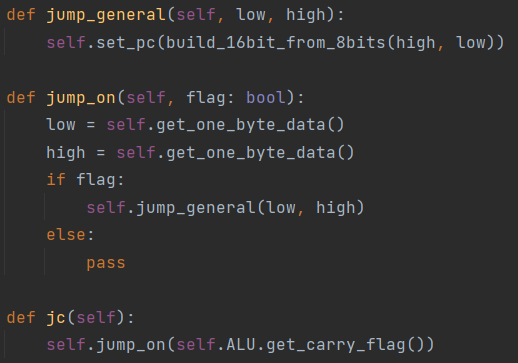
\includegraphics[width=10cm]{Bilder/JumpVariants}
\label{fig:JumpVariants}
\end{figure}


\subsubsection{Binäre Addition uns Subtraktion}
Da die Additions- und Subtraktions-Befehle das Carry- und Auxiliary-Carry-Flag verändern, musste eine manuelle Addition implementiert werden. Das Carry-Flag, das anzeigt, ob ein Überlauf beim siebten Bit stattgefunden hat, hätte noch ohne eine eigene Implementierung der Addition funktioniert. Dafür müsste nur vor dem Casten in einen 8-Bit Wert überprüft werden, ob der Wert größer als 255 ist. Da aber zusätzlich noch das Auxiliary-Carry-Flag beachtet werden musste, dass einen Überlauf von Bit 3 anzeigt, wurde die Addition selber implementiert. Diese Implementierung liefert das Carry-, Auxiliary-Carry-Flag und das Ergebnis der Addition. Somit können die Flags korrekt gesetzt werden sofern die Befehle diese Flags ändern. Sofern eines der beiden Flags verändert wird, wird darauf zurückgegriffen. Der INX-Befehl, der einen 16-Bit Wert um 1 erhöht, verändert aber keine Flags, weshalb dort eine normale Addition durchgeführt wird.
\imgSpaceBefore
\begin{figure}[H]
\caption{Implementierung der binären Addition}
\centering
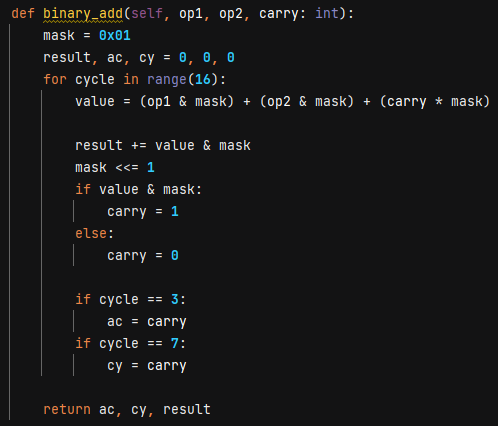
\includegraphics[width=10cm]{Bilder/binaere_addition}
\label{fig:binaere_addition}
\end{figure}


\subsubsection{GUI-Methoden}
Die eine Seite des Simulators ist das Simulieren des Prozessors, mit diesem muss aber auch interagiert werden. Die in diesem Abschnitt erklärten Funktionen beziehen sich deshalb auf die in \ref{chp:AufbauGUI} beschriebenen Funktionen für die Benutzeroberfläche.


\subsection{Single-Prozessor-Simulator}
\label{SPS_impl}
Von Andreas
\\

In diesem Kapitel wird gezeigt, was die neue Version des Simulator kann. Dieser unterscheidet sich in sofern von dem Multi-Prozessor-Simulator, dass jeder Befehl aus mehreren Maschinen Zyklen und diese wiederum aus mehreren Zuständen bestehen. So ist es möglich, komplette Befehle aber auch einzelne Maschinen Zyklen oder sogar Zustände auszuführen. Damit kann wesentlich besser nachvollzogen werden, wie ein Prozessor tatsächlich funktioniert. In der Multi-Prozessor-Variante konnten zwar Programme ausgeführt werden, aber wie die Befehle ausgeführt worden sind, war weit weg von der Funktionsweise eines echten Prozessors. 

\subsubsection{Aufbau eines Befehls}

Jeder Befehl besteht aus einem Array von Maschinen Zyklen. Zusätzlich enthält jeder Befehl auch einen Zähler, wie viele Maschinen Zyklen, der Befehl schon ausgeführt hat. Ein Befehl hat auch nur eine wichtige Methode. Die next\_state()-Methode sorgt dafür, dass der aktuelle Maschinen Zyklus seine next\_state()-Methode ausführt. Wenn die Maschinen Zyklus next\_state()-Methode True zurückliefert, bedeutet das, dass der letzte Zustand des Maschinen Zyklus ausgeführt wurde. Wenn dies der Fall ist, wird der Maschinen Zyklus Zähler um eins erhöht und es wird ebenfalls ein True zurückgeliefert. Dieses Signal des Maschinen Zyklus wird bis in die äußerste Schicht weitergeleitet, damit dort spezielle Ereignisse ausgeführt werden können z.B. die GUI aktualisieren. Beim nächsten Aufruf von next\_state() wird somit der erste Zustand des nächsten Maschinen Zyklus ausgeführt.
\\

\noindent
Jeder Maschinen Zyklus besteht aus einem Array von Zuständen, einem Zähler, der die bisher ausgeführten Zustände zählt und eine Referenz auf den Prozessor. Diese Referenz ist notwendig, damit die Zustände, die in den Maschinen Zyklen ausgeführt werden, den Prozessor verändern und dessen Methoden verwenden können. Die next\_state()-Methode führt immer die run()-Methode der Zustände aus und erhöht seinen Zähler um eins. Wenn der eben ausgeführte Zustand der letzte im Maschinen Zyklus war, wird der Zähler zurückgesetzt und ein True zurückgegeben.
\\

\noindent
Ein Zustand besitzt nur eine Referenz zum Prozessor und eine run()-Methode, die den Zustand ausführt. Da ein Zustand zu allen möglichen Stellen in einem Maschinen Zyklus verwendet werden kann, besitzt der Zustand selber keine weiteren Informationen.


\subsubsection{Programmablauf}

Wie bei der ersten Version dieses Simulator, wird ein .com-Datei benötigt um ein Programm ausführen zu lassen. Über die GUI kann eine solche Datei eingelesen werden. Damit wird wieder der Programmspeicher befüllt.
Die GUI besitzt vier Knöpfe, die das ausführen eines Befehls/Maschinen Zyklus oder Zustand auslöst. Bei dem \glqq Next State\grqq -Knopf wird genau ein Zustand ausgeführt. Bei dem \glqq Next Machine Cycle\grqq -Knopf wird der aktuelle Maschinen Zyklus bis zum Schluss ausgeführt. Der  \glqq Next Instruction\grqq -Knopf verhält sich wie der Maschinen Zyklus-Knopf. Der \glqq Go\grqq -Knopf führt zu solange den nächsten Zustand aus bis der Knopf wieder gedrückt wird. Die drei ersten Knöpfe sind auf eine Methode im Intel8080 gebunden, die den selben Namen tragen wie der Knopf. Jeder dieser Methoden gibt True zurück, wenn der nächste auszuführende Zustand zu einem neuen Befehl gehört. 
Die next\_instruction()-Methode führt solange die next\_machine\_cycle()-Methode aus, bis diese True zurückliefert. Diese wiederum führt solange die next\_state\_internal()-Methode aus, bis diese True zurückliefert. Diese liefert True, wenn der letzte Zustand eines Maschinen Zyklus ausgeführt wurde. Die next\_state()-Methode ruft nur einmal die next\_state\_internal()-Methode auf.

Die next\_state\_internal()-Methode steuert wann ein neuer Befehl dekodiert und eine neue Klasse geladen werden muss. Wenn der nächste Zustand der erste eines neuen Befehls ist, wird der current\_instruction-Variable ein Nop-Befehl zugewiesen. Da bei allen Befehlen, die ersten drei Zustände die gleichen sind, ist es nicht wichtig welcher Befehl hier geladen wird. Erst im dritten Zustand wird der tatsächliche Befehl geladen. Von diesem Befehl wird der zuletzt ausgeführten Zustand auf drei gesetzt. Wenn der letzte Zustand eines Maschinen Zyklus ausgeführt wurde wird True zurückgegeben. Wenn ein Befehl frühzeitig abgebrochen werden soll, also z.B. bei einem bedingten Sprung, wird das ebenfalls hier gemacht.

\subsubsection{Dekodieren eines Befehls}
Bei jedem Fetch Zyklus wird das aktuelle Befehlsbyte in die cpu\_insturction\_register-Variable geschrieben. Ähnlich wie bei der ersten Version, wird beim Dekodieren dieses Byte mit Hexadezimalen Werten verglichen. Bei dieser Version wird beim dekodieren aber ein Unterschied gemacht bei Befehlen, die entweder ein Register oder eine Adresse als Parameter erhalten (siehe Abbildung \ref{fig:Decode_instr}). Dies ist deswegen wichtig, da sich die Maschinen Zyklen davon unterscheiden. Abbildung \ref{fig:ReadInstruction}  zeigt, dass in der ersten Version für alle ADD Befehle nur eine Methode aufgerufen wird. Damit der Prozessor die richtigen Klassen zur Ausführung verwendet, wird in der current\_instruction-Variable ein Objekt des richtigen Befehls gespeichert.
\imgSpaceBefore
\begin{figure}[H]
\caption{Implementierung der Dekodierung}
\centering
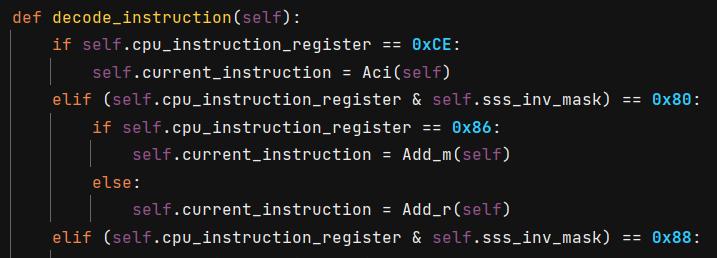
\includegraphics[width=15cm]{bilder/DecodeInstruction}
\label{fig:Decode_instr}
\end{figure}

\subsubsection{Programmaufbau}

Der Simulator besteht immer noch hauptsächlich aus dem Prozessor, der ALU und den Registern. Dadurch, dass aber jeder Befehl, Maschinen Zyklus und Zustand eine eigene Klasse  hat gibt es nun wesentlich mehr Klassen. Insgesamt gibt es:
\begin{itemize}
\item 73 Befehls-Klassen
\item 84 Maschinen Zyklen-Klassen
\item 100 Zustands-Klassen
\end{itemize}

\noindent
Zusätzlich dazu gibt es nochmal ungefähr 10 Klassen, von denen die oben genannten abgeleitet sind.

\noindent
Der in Kapitel \ref{chapter:MPS_aufbau} gezeigte DCX Befehl sieht nun folgendermaßen aus.
\imgSpaceBefore
\begin{figure}[H]
\caption{DCX Befehl und Maschinen Zyklus}
\centering
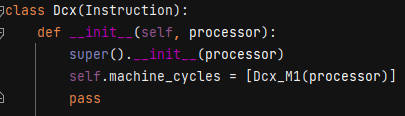
\includegraphics[width=15cm]{bilder/dcx_inst}
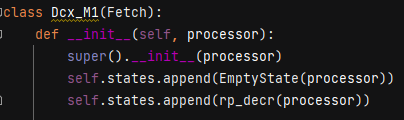
\includegraphics[width=15cm]{bilder/dcx_mc}
\label{fig:Dcx_instr}
\end{figure}

\noindent
Bei vielen Befehlen werden leere Zustände verwendet. Das kommt daher, dass es mit dem Simulator momentan nicht möglich einen Zustand zu erstellen, der zwei Takte dauert. Deshalb wird mit dem ersten Takt ein leerer Zustand ausgeführt und im zweiten dann erst der eigentliche Zustand. Somit werden die Daten zur gleichen Zeit in die Register/Speicher geschrieben, wie es bei einem richtigen Prozessor auch der Fall ist.
\imgSpaceBefore
\begin{figure}[H]
\caption{DCX (rp\_decr) Zustand}
\centering
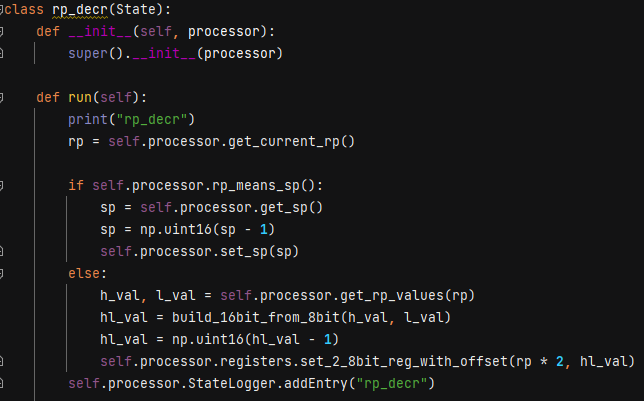
\includegraphics[width=15cm]{bilder/dcx_state}
\label{fig:Dcx_state}
\end{figure}

\noindent
Da der DCX Befehl nur aus einem Maschinen Zyklus, und mit dem leeren Zustand nur über einen Zustand verfügt, der den Befehl ausmacht werden im folgenden nochmal anderen Befehle gezeigt, bei denen diese Klassenstruktur mehr Sinn ergibt. Im folgenden Kapitel werden weitere Befehle angeschaut, die auch zeigen, wie in der neuen Version Befehle des gleichen Typs auf die selben Maschinen Zyklen und Zustände zurückgreifen.


\subsubsection{Befehlsvarianten}
Alle Befehle haben die gleichen ersten drei Zustände. Deswegen wurde auch ein Fetch-Maschinen Zyklus erstellt, wovon jeder erste Maschinen Zyklus abgeleitet wurde. Der RST-Befehl hat, als einzige Ausnahme, einen anderen dritten Zustand. Normalerweise wird im dritten Zustand nur der aktuelle Befehl in das Befehls Register geschrieben. Beim RST-Befehl wird aber zusätzlich noch das W-Register auf Null gesetzt. Dies ist deswegen wichtig, da der Befehl an eine von acht Programmstellen springen soll. Diese liegen alle am Anfang des Programmspeichers und benötigen deswegen ein leeres W-Register. Für Sprünge werden das W- und Z-Register verwendet. In den Maschinen Zyklen 2-4 wird aber nur das Z-Register auf den entsprechenden Wert gesetzt.
\\

\noindent
Bei einigen Befehlen gibt es grundsätzlich drei verschiedene Typen, die unterschieden werden. Einen direkten Befehl, der ein weiteres Byte hinter dem Befehl im Programmspeicher liest, einen Befehl, der einen Register-Wert liest, im restlichen Kapitel als Register-Befehl bezeichnet, und einen Befehl, der zuerst die zwei folgenden Bytes aus dem Programmspeicher liest, daraus eine Adresse bildet und dann an diese Adresse springt und den dort liegenden Wert verwendet. Im restlichen Kapitel an Speicher-Befehl bezeichnet.


\begin{table}[H]
\centering
\caption{Befehle mit diesen drei Befehls-Typen}
\label{table:instr_types}
\begin{tabular}{|l|c|c|c|c| } 
 \hline
 Beschreibung & Register-Befehl & Speicher-Befehl & Direkter Befehl \\
 \hline 
 Addition mit Acc & ADD r & ADD m & ADI \\ 
 Addition mit Acc \& Cy & ADC r & ADC m & ACI \\ 
 Subtraktion mit Acc & SUB r & SUB m & SUI \\ 
 Subtraktion mit Acc \& Cy & SBB r & SBB m & SBI \\ 
 Bitweise UND-Operation & ANA r & ANA m & ANI \\ 
 Bitweise XOR-Operation & XRA r & XRA m & XRI \\ 
 Bitweise ODER-Operation & ORA r & ORA m & ORI \\ 
 Vergleich mit Acc & CMP r & CMP m & CPI \\ 
 \hline
\end{tabular}
\end{table}

\noindent
Für die Addition ohne Carry gibt es diese drei Typen. ADD r verwendet ein Register. ADD m verwendet einen Wert, der irgendwo im Programmspeicher liegt und der ADI-Befehl verwendet das zweite Byte des Befehls als Summand. Alle drei Befehle müssen das Gleiche machen. Einen Wert mit dem Akkumulator addieren. Dazu nutzt jeder Befehl aber Werte von unterschiedlichen Stellen und müssen diese unterschiedlich laden. 
Als letzter Maschinen Zyklus addieren alle diese drei Befehle das ACT- und TMP-Register ohne Carry. Das Ergebnis wird am Ende immer in den Akkumulator geschrieben. Deswegen hat jeder dieser Befehle als letztes den Add\_MC Maschinen Zyklus. 
In das ACT-Register wird immer der ursprüngliche Wert des Akkumulators geladen. Der Unterschied der Befehle ist nur, dass in den vorherigen Maschinen Zyklen, andere Werte in das TMP-Register gespeichert werden (siehe Tabelle \ref{table:mc_types}). 
\\

\noindent
\textbf{Unterschiede des ersten Maschinen Zyklus}

\noindent
Der direkte Befehl und der Speicher-Befehl besitzen den gleichen ersten Zustand. Dort wird einfach nur der Inhalt des Akkumulators in das ACT-Register geschrieben.
Der Register-Befehl kann im ersten Maschinen Zyklus sowohl den Wert des Akkumulators in das ACT-Register, als auch das im Befehl kodierte Register in das TMP-Register laden.
\\

\noindent
\textbf{Unterschiede des zweiten Maschinen Zyklus}

\noindent
Der Register-Befehl, hat im ersten Zyklus schon beide Register so vorbereitet, dass er im zweiten Zyklus diese Werte bereits addieren kann. Für diesen Befehlstyp ist das schon der letzte Zyklus.
Die beiden anderen Befehle müssen zuerst noch das TMP-Register mit dem korrekten Wert laden. Der direkte Befehl muss dafür erst noch den Programmzähler um eins erhöhen, damit das folgende Byte ausgelesen werden kann. Der Speicher-Befehl lädt den Wert, an der angegebenen Adresse, direkt in das TMP-Register.
\\

\noindent
\textbf{Unterschiede des dritten Maschinen Zyklus}

\noindent
Der Register-Befehl führt keinen dritten Zyklus aus.
Der direkte Befehl und der Speicher-Befehl führen jetzt den gleichen Maschinen Zyklus aus, der der Register-Befehl schon im zweiten Zyklus ausgeführt hat.

\begin{table}[H]
\centering
\caption{Maschinen Zyklen der unterschiedlichen Typen}
\label{table:mc_types}
\begin{tabular}{|l|c|c|c|c| } 
 \hline
 Befehls-Typ & 1. Zyklus & 2. Zyklus & 3. Zyklus \\
 \hline 
 Register-Befehl
 &
 \begin{lstlisting}
(SSS) $\rightarrow$ TMP
 \end{lstlisting}
 &
 \begin{lstlisting}
ADD$\_$MC
 \end{lstlisting}
 & \\
 
 Speicher-Befehl & 
 \begin{lstlisting}
(ACC) $\rightarrow$ ACT 
 \end{lstlisting}  
  & 
 \begin{lstlisting}
Data   $\rightarrow$ TMP 
 \end{lstlisting} 
 & 
 \begin{lstlisting}
ADD_MC
 \end{lstlisting} 
 \\ 
 
 Direkter Befehl & 
 \begin{lstlisting}
(ACC) $\rightarrow$ ACT 
 \end{lstlisting} 
 & 
 \begin{lstlisting}
Byte 2 $\rightarrow$ TMP
 \end{lstlisting} 
 &
  \begin{lstlisting}
ADD_MC
 \end{lstlisting}
 \\
 
 \hline
\end{tabular}
\end{table}


\subsubsection{Besonderheiten des Simulators}
Bei der Entwicklung dieses Simulators wurde vieles, was ein echter Prozessor macht, nicht implementiert. In diesem Kapitel soll aufgezeigt werden, welche Unterschiede es zu einem echten Prozessor gibt.
\\

\noindent
\textbf{Adress- und Datenbus}

\noindent
Der Intel 8080 besitzt einen 8-Bit Daten- und einen 16-Bit Adressbus. 
In diesem Simulator wurde kein einziger Bus implementiert. Grund dafür ist, dass die Busse anhand von verschiedenen Taktgebern, beschrieben und gelesen werden. Dies könnte zwar auch simuliert werden, letztendlich haben aber wir uns aber dagegen entschieden, da dies keine nennenswerte Vorteile bietet und den Simulator in ein weitere Richtung wesentlich komplexer macht. Einer der wenigen Gründe warum es doch Sinn gemacht hätte Busse zu verwenden wäre, dass auf dem Adress- und Datenbus die Daten zu sehen wären, die darüber gesendet werden. Dadurch, dass aber nach jedem Zustand die Daten irgendwo gespeichert werden, können die Veränderungen direkt beobachtet werden. Zwar wäre es schön gewesen, wenn die Daten aus dem Programmspeicher über die Busse laufen würden, aber für einen Simulator ist das nicht zwangsweise notwendig. Normalerweise wird auch über diese Busse mit dem Programmspeicher kommuniziert. Dies wurde in diesem Simulator aber umgangen, indem der Prozessor direkten Zugriff auf den Speicher hat. Generell werden die Busse dazu verwendet, um mit externen Geräten zu kommunizieren. Da dieser Simulator aber nicht dafür gedacht ist, wurden diese komplett weggelassen. Deswegen wurden für den In- und Out-Befehl der letzte Zyklus nur mit leeren Zuständen gefüllt. So brauchen diese Befehle immer noch die vorgesehenen Anzahl an Zuständen, lesen und schreiben aber keine Daten.
\\

\noindent
In jedem ersten Zustand aller Maschinen Zyklen wird über den Datenbus ein 8-Bit Status Wort gesendet. Damit lässt sich erkennen welche Art von Maschinen Zyklus ausgeführt wird. 
Die notwendigen Zustände existieren dafür, schreiben aber nichts in den Bus. Zum einen, da es keinen Bus gibt und zum Anderen, da in der Beschreibung der Zustände (siehe Anhang \ref{anhang:instr_state}) nur so viel steht wie \glqq PC OUT STATUS\grqq im ersten Zustand des Fetch Zyklus. Daraus ist nicht direkt ableitbar was auf den Datenbus geschrieben werden soll. In Abbildung \ref{fig:status_word} ist zu sehen, wie die verschiedenen Zustände auf dem Bus codiert werden würden. So wird ein Memory Write Zyklus dadurch bestimmt, dass alle Datenbits d\textsubscript{0-7} auf Null gesetzt werden.

\begin{figure}[H]
\caption{Kodierung der Befehlstypen beim SYNC Takt}
\centering
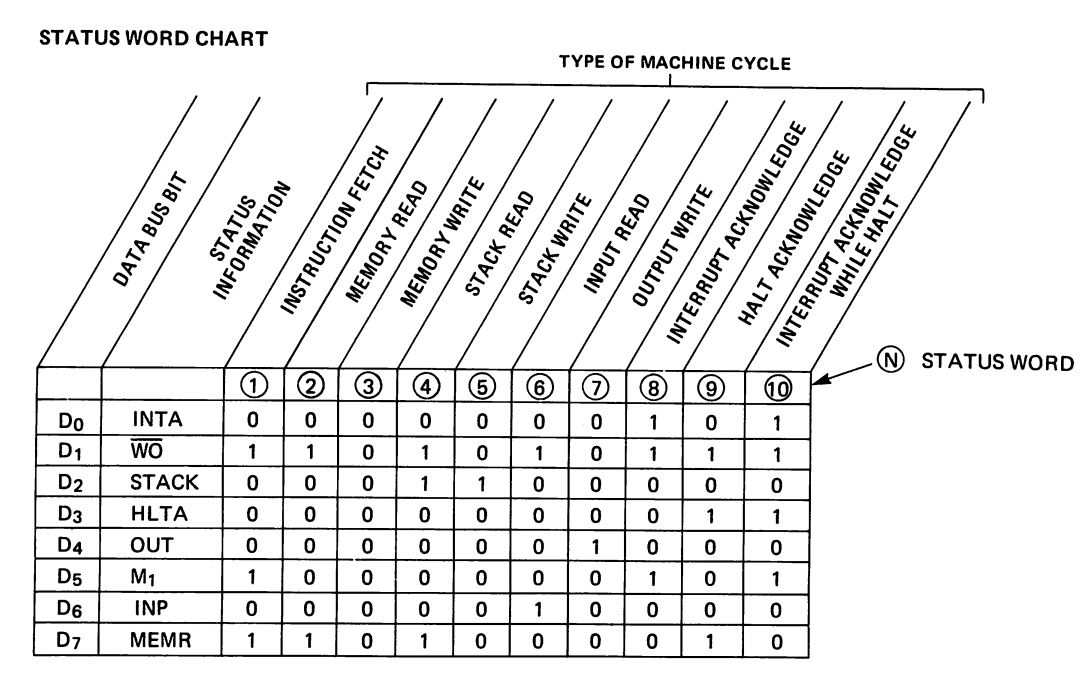
\includegraphics[width=15cm]{Bilder/Intel8080_DataLines}
\label{fig:status_word}
\end{figure}

\textbf{
keine zwei takt zustände, kein halt, kein paralleles ausführen, Mc 6 nicht als Fetch des nächsten Befehls, nur positive werte, mvi pc + 1, ALU->ddd nicht verwendet, die meisten ersten Zustände machen nichts da sie Infos auf den lines ausgeben, daten bus nicht verwendet
}

\newpage

\section{Fazit und Ausblick}
Platzhalter

\newpage


\addcontentsline{toc}{section}{Literatur}
\begin{thebibliography}{9}
\bibitem{Beispiel}
Google: \url{https://www.google.com}
\bibitem{Grundlagen der Informatik}
Grundlagen der Informatik: Herold, Lurz, Wohlrab und Hopf; 3. aktualisierte Auflage (2017), Pearson
\bibitem{Adressformate}Instruction formats: \url{https://www.geeksforgeeks.org/computer-organization-instruction-formats-zero-one-two-three-address-instruction/}, zuletzt abgerufen: 25.12.2021
\end{thebibliography}



%\newpage
%\thispagestyle{empty}
%
%\section*{Anhang}
%\addcontentsline{toc}{section}{Anhang}


\end{document}
